%\documentclass[12pt,a4paper]{article} % POUR TEST
%\usepackage[french]{babel} % POUR TEST
%\usepackage[latin1]{inputenc} % POUR TEST
%\usepackage[T1]{fontenc} % POUR TEST
%\usepackage{vmargin} % POUR TEST
%\usepackage{pdfpages} % POUR TEST
%\setmarginsrb{2.5cm}{1.5cm}{2.5cm}{2cm}{0cm}{0cm}{0cm}{0cm} % POUR TEST

%\begin{document} % POUR TEST
\pagestyle{empty}
{\sffamily
\noindent{Universit\'{e} de Lille \hfill Facult\'{e} de Pharmacie de Lille \\ Ann\'{e}e Universitaire 2022/2023}

\vspace{25mm}
\begin{center}
\textbf{THESE \\
POUR LE DIPLOME D'ETAT \\
DE DOCTEUR EN PHARMACIE}
\end{center}
\vspace{13mm}
\noindent{\textbf{\hspace*{13mm}Soutenue publiquement le 12 septembre 2023 \\
\hspace*{13mm}Par M. RIHANI Emir Ka\"{i}s}}
\vspace{26mm}
\begin{center}
\rule{65mm}{0.8pt} \\
\vspace{6mm}
\textbf{APPLICATION DE MODELES D'APPRENTISSAGE MACHINE \\~\\ A LA CLASSIFICATION DES MACROMYCETES} \\
\vspace{2mm}
\rule{65mm}{0.8pt}
\end{center}
\vspace{45mm}
\noindent{\textbf{\underline{\smash{Membres du jury}} :} \\
~\\
\textbf{Pr\'{e}sident :} Nom, Prenom, titre et lieu de fonction \\
~\\
%\textbf{Directeur, conseiller de th\`{e}se :} Dr \textsc{Hamonier} Julien, Maître de Conférences en Biomathématiques \\
\textbf{Directeur de th\`{e}se :} Dr \textsc{Hamonier} Julien, Maître de Conférences en Biomathématiques \\
~\\
\textbf{Assesseur(s) :} Nom, Prenom, titre et lieu de fonction}
}
\newpage
~ % page blanche verso de couverture

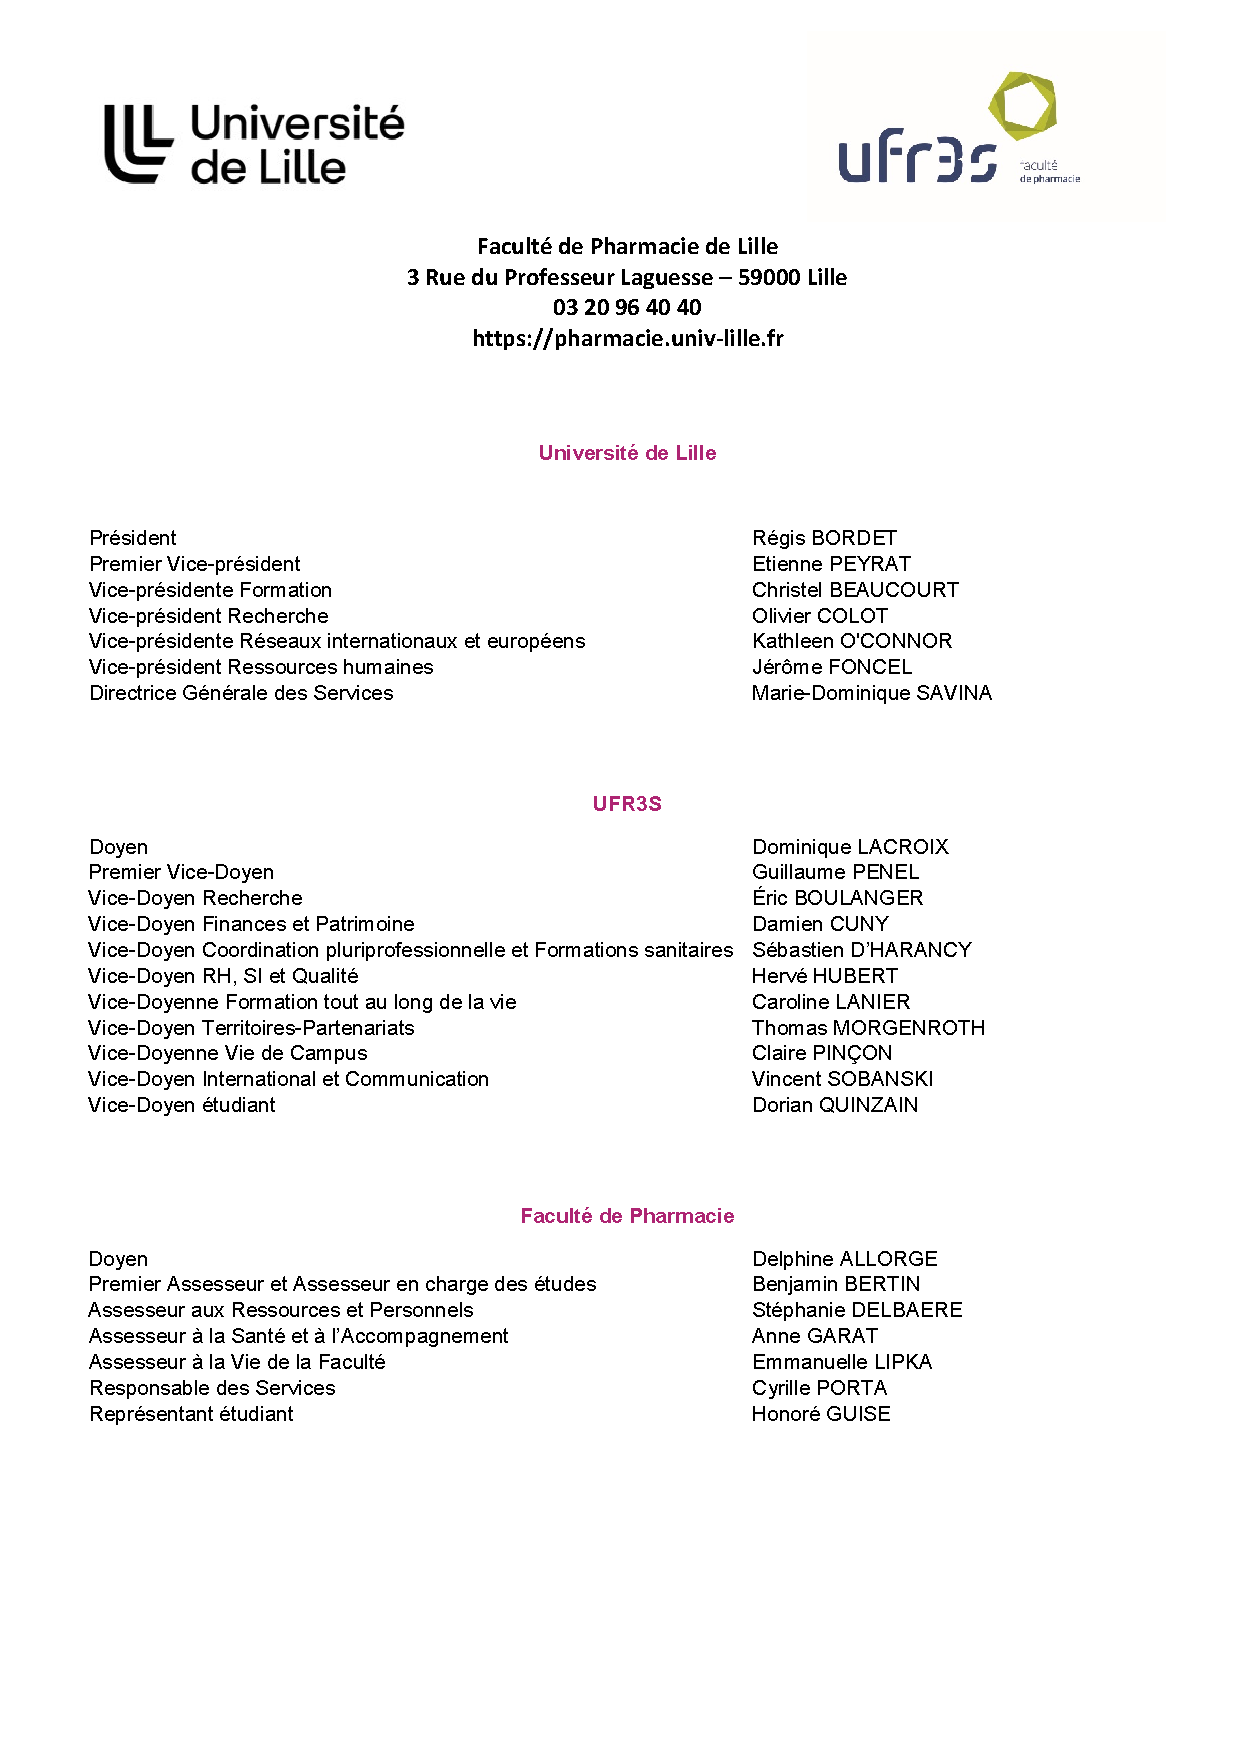
\includepdf[pages={-}]{fac-enseignants2022.pdf} % liste des profs
\newpage
~ % page blanche verso liste des profs

\newpage
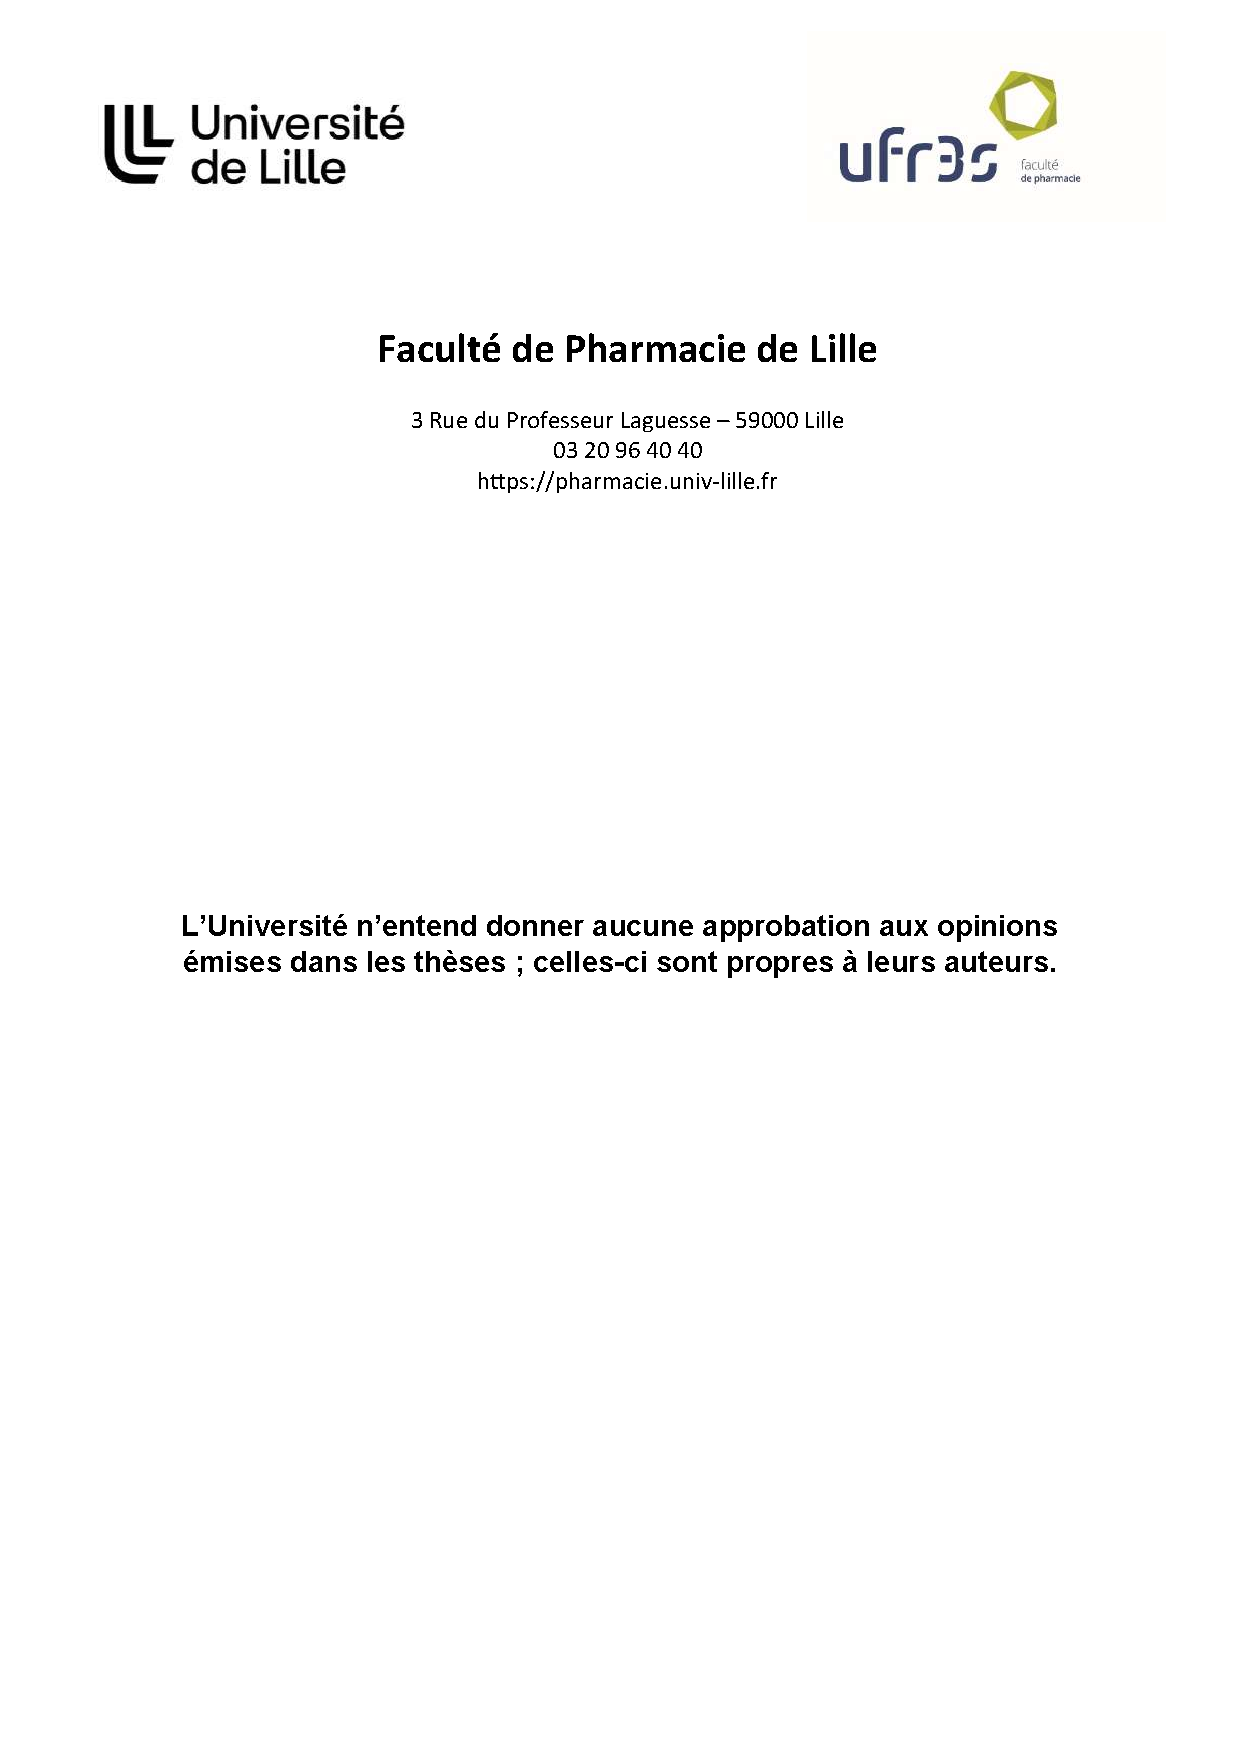
\includepdf[pages={-}]{fac-disclaimer.pdf} % disclaimer opinions
\newpage
~ % page blanche verso disclaimer

\newpage
{\rmfamily
~ \\ ~
\vspace{2cm}
{\itshape J'adresse mes sinc\`{e}res remerciements \`{a} :
\vspace{2cm}
\paragraph*{}
La Dream Team de tous ceux que je vais remercier
}
}
\newpage
~ %page blanche verso de remerciements

\newpage %début document (sommaire)
%\end{document} % POUR TEST
